%; whizzy paragraph -pdf xpdf -latex ./whizzypdfptex.sh
%; whizzy-paragraph "^\\\\begin{frame}"
% latex beamer presentation.
% platex、 latex-beamer でコンパイルすることを想定。 

%     Tokyo Debian Meeting resources
%     Copyright (C) 2009 Junichi Uekawa
%     Copyright (C) 2010 Nobuhiro Iwamatsu

%     This program is free software; you can redistribute it and/or modify
%     it under the terms of the GNU General Public License as published by
%     the Free Software Foundation; either version 2 of the License, or
%     (at your option) any later version.

%     This program is distributed in the hope that it will be useful,
%     but WITHOUT ANY WARRANTY; without even the implied warranty of
%     MERCHANTABILITY or FITNESS FOR A PARTICULAR PURPOSE.  See the
%     GNU General Public License for more details.

%     You should have received a copy of the GNU General Public License
%     along with this program; if not, write to the Free Software
%     Foundation, Inc., 51 Franklin St, Fifth Floor, Boston, MA  02110-1301 USA

\documentclass[cjk,dvipdfmx,12pt]{beamer}
\usetheme{Tokyo}
\usepackage{monthlypresentation}

%  preview (shell-command (concat "evince " (replace-regexp-in-string "tex$" "pdf"(buffer-file-name)) "&"))
%  presentation (shell-command (concat "xpdf -fullscreen " (replace-regexp-in-string "tex$" "pdf"(buffer-file-name)) "&"))
%  presentation (shell-command (concat "evince " (replace-regexp-in-string "tex$" "pdf"(buffer-file-name)) "&"))

%http://www.naney.org/diki/dk/hyperref.html
%日本語EUC系環境の時
\AtBeginDvi{\special{pdf:tounicode EUC-UCS2}}
%シフトJIS系環境の時
%\AtBeginDvi{\special{pdf:tounicode 90ms-RKSJ-UCS2}}

\title{東京エリアDebian 出張勉強会}
\subtitle{資料}
%\author{荒木 靖弘 ar@debian.org\\IRC nick: ar}
\author{岩松 信洋 iwamatsu@debian.org\\IRC nick: iwamatsu}
\date{2010年06月26日}
\logo{
\includegraphics[width=8cm]{image200607/openlogo-light.eps}}

\begin{document}

\frame{\titlepage{}}


%\begin{frame}{本日のアジェンダ}
% \begin{enumerate}
%  \item Debian とは \\ 担当: 荒木 靖宏
%  \item あなたはどっち、CloudでDebian、 DebianでCloud \\ 担当: 荒木 靖宏
%  \item Squeeze に向けた Debian GNU/kFreeBSD 入門\\ 担当: 岩松 信洋
% \end{enumerate}
%\end{frame}

%\begin{frame}{あなたはどっち、CloudでDebian, DebianでCloud}
%\end{frame}

\emtext{Squeeze に向けた Debian GNU/kFreeBSD 入門}

\begin{frame}{本日のアジェンダ}
 \begin{enumerate}
  \item 自己紹介
  \item Debian GNU/kFreeBSD って何?
  \item なぜ kFreeBSDなの?
  \item Debian GNU/Linux との違い
  \item Debian GNU/kFreeBSD を使うメリット
  \item まとめ
 \end{enumerate}
\end{frame}

\section{自己紹介}
\begin{frame}{自己紹介}
 \begin{itemize}
  \item 名前: 岩松 信洋(いわまつ のぶひろ)
  \item Debian Project Official Developer
  \item Debian : USB カメラ、 OpenCV , Bluetooth メンテナ。
  Renesas SH/SH4 Porter, Buildd メンテナ。
  \item 普段: ブートローダの開発、Linuxカーネルの開発、ユーザアプリケーション、Webアプリケーションの開発など。
  \item なぜか毎年 OSC/北海道 に呼ばれてる。(去年はgitハンズオンしていました。)
 \end{itemize}
\end{frame}

\begin{frame}{Debian GNU/kFreeBSDって何?}

\end{frame}

\begin{frame}{Debian GNU/kFreeBSDって何?}
  \begin{itemize}
    \item<1-> Debian の移植版のひとつ。1999年ごろから開発が開始。\\

ただし、そのころは妄想のみ。数年後、glibcへの移植が開始される。
    \item<2-> 次期リリースからDebianオフィシャルアーカイブに取り込まれる予定。
          今までは debian-ports で開発及び公開。
    \item<3-> アーキテクチャは2つ。kfreebsd-i386 と kfreebsd-amd64。
  \end{itemize}
\end{frame}

\begin{frame}{なぜkFreeBSDなの?}

\end{frame}

\begin{frame}{なぜkFreeBSDなの?}
\sout{なぜこんなバカなことをするの?}\\
なぜ、kFreeBSDなの?
\end{frame}

\begin{frame}{再確認}
\begin{itemize}
\item<1-> Debian ProjectはフリーなOSを作る団体であーる!キリッ!
\item<2-> Debian は Linuxカーネルに特化していない。
\item<3-> LinuxカーネルをFreeBSDカーネルに置き換えようとしているわけではない。
\item<4-> カーネルに依存しないユニバーサルOSを作る。
\end{itemize}
\end{frame}

\begin{frame}{Debian OSの簡単な構造}
\includegraphics[width=0.7\hsize]{image201006/os-block01.eps}
\end{frame}


\begin{frame}{Debian OSの簡単な構造}
\includegraphics[width=1.0\hsize]{image201006/os-block01-1.eps}
\end{frame}


\begin{frame}{Debian OSの簡単な構造}
\includegraphics[width=1.0\hsize]{image201006/os-block01-2.eps}
\end{frame}


\begin{frame}{Debian OSの簡単な構造}
\includegraphics[width=1.0\hsize]{image201006/os-block01-3.eps}
\end{frame}

%\begin{frame}
%\begin{itemize}
%\item<1-> Debian: DFSG, dpkg, apt, Debian パッケージ, インストーラ
%\item<2-> GNU: eglibc(glibc), Userland (gcc, coreutils, etc)
%\item<3-> kFreeBSD: FreeBSD-Kernel / 7.3 と 8.0
%\end{itemize}
%\end{frame}

\begin{frame}{Debian GNU/Linux の場合}
\includegraphics[width=0.8\hsize]{image201006/os-block02.eps}
\end{frame}

\begin{frame}{Debian GNU/kFreeBSD の場合}
\includegraphics[width=0.8\hsize]{image201006/os-block03.eps}
\end{frame}

\begin{frame}{Debian GNU/kFreeBSD}
\begin{center}

\includegraphics[width=0.5\hsize]{image201006/debian-kfreebsd.png}\\
kernel が FreeBSDだから、 kFreeBSD。
\end{center}
\end{frame}

\begin{frame}{Debian GNU/Linux との違い}

\end{frame}

\begin{frame}{Debian GNU/Linux との違い}
\begin{itemize}
\item<1-> ALSA 関連 \\
kFreeBSD では ALSAではなく、OSSを使う。
\item<2-> Video 4 Linux 関連
\item<3-> Bluetooth 関連\\
スタックとツールが異なる。絶賛開発中。
\item<4-> セキュリティ関連 \\
selinux, tomoyo, etc.
\item<5-> Linux ドライバ 関連
\item<6-> その他、細かいもの\\
libiw, inotify, etc.. 
\item<7-> あとは同じ!ヒャッホー!
\end{itemize}
\pause
\end{frame}


\begin{frame}[containsverbatim]{簡単なポーティング例}
簡単なポーティングの例を紹介\\
\begin{minipage}[t]{0.45\hsize}
悪い例
\begin{commandline}
#ifdef __linux__
#include <endian.h>
#elif __FreeBSD__
#include <sys/endian.h>
#else
#error ``Unknown system''
#endif
\end{commandline}
\end{minipage}
\begin{minipage}[t]{0.45\hsize}
良い例
\begin{commandline}
#ifdef __GLIBC__
#include <endian.h>
#elif __FreeBSD__
#include <sys/endian.h>
#else
#error ``Unknown system''
#endif
\end{commandline}
\end{minipage}

Linux はカーネルですよ....。\texttt{\_\_GLIBC\_\_}に変えましょう。
\end{frame}

\begin{frame}{Debian GNU/kFreeBSDを使うメリット}

\end{frame}

\begin{frame}{Debian GNU/kFreeBSDを使うメリット}
\begin{itemize}
\item<1-> カーネルは FreeBSD で Debian のシステムが使える!
\item<2-> カーネルは FreeBSD で GNUのソフトウェアが使える!
\item<3-> カーネルは FreeBSD で DFSG フリーな環境が構築できる!\\
元のkFreeBSDには再配布に問題のあるバイナリドライバが含まれる。
Freeじゃない! 
\end{itemize}
\end{frame}

\begin{frame}{Debian GNU/kFreeBSDを使うメリット}
\begin{itemize}
\item jail 
\item ZFS\\
CDDLによって、ext2fs.ko や zfs.ko とは同時に使えない。\\
ユーザランドツールがまだない。\\
\item OpenBSD Packet Filter (pf)
\item dtrace 
\item NDIS
\end{itemize}
\end{frame}

\begin{frame}{実際使っている人いるの?}
実際使っている人いるの? \\
\pause
いねーだろ、プギャー!\\
\pause
\begin{center}
\color{red}

残念!\\
プレゼンマシンは Debian GNU/kFreeBSD が動いています。
\end{center}
\end{frame}

\begin{frame}{実際使っている人いるの?}
\begin{itemize}

\item \url{http://popcon.debian.org}によると
世界に最低36台ぐらい使われているらしい。

\item そのうちの一台が埼玉県の所沢ぐらいにあるらしい。
\item ちなみに amd64 は最低25182台。
\end{itemize}

\end{frame}

\begin{frame}{実際使っている人いるの?}
ここ、1ヶ月ほどDebian GNU/kFreeBSD上で生活してみた。
\begin{itemize}
\item<1-> インターネット、OOo など、問題なく動作する。
\item<2-> gcc を使った開発も特に特に問題なし。
\item<3-> GtkなどのGUI tool kit を使った開発も特に問題なし。
\end{itemize}
\end{frame}

\begin{frame}{ベンチマーク}
ベンチマーク\\
\url{http://www.phoronix.com/scan.php?page=article\&item=debian_kfreebsd\&num=1}
\end{frame}

\begin{frame}{まとめ}

\end{frame}

\begin{frame}{まとめ}
\begin{itemize}
\item<1-> 普段使う分には問題ない。\\
インターネット、OOo。
\item<2-> 開発も普通にできる。\\
\item<3-> 一家に一台、Debian GNU/KFreeBSDマシン
\end{itemize}
\end{frame}


\begin{frame}{その他情報/参考資料}
\begin{itemize}
\item \url{http://wiki.debian.org/Debian\_GNU/kFreeBSD}
\item \url{http://wiki.debian.org/Debian\_GNU/kFreeBSD\_FAQ}
\item メーリングリスト: http://lists.debian.org/debian-bsd/
\item IRC: \#debian-kbsd at irc.debian.org
\item \url{svn.schmehl.info/svn/talks/kfreebsd/trunk/debian-kfreebsd.pdf}
\end{itemize}
\end{frame}

\begin{frame}{この資料}
\begin{itemize}
\item 東京エリアDebian勉強会ページで公開されています。\\
\url{http://tokyodebian.alioth.debian.org/2010-06-osc2010-do.html}

\end{itemize}
\end{frame}

\begin{frame}{GPGキーサインパーティ}
\begin{itemize}
\item 昼 12:05 からGPGキーサインパーティやります。\\
興味のある方は 岩松 まで。
\end{itemize}
\end{frame}



\begin{frame}{次回の勉強会}

\begin{itemize}
 \item 2010年7月17日: 東京 荻窪
 \item 2010年8月1日 - 7日 : アメリカ ニューヨーク、コロンビア大学
\end{itemize}
 
\end{frame}

\end{document}

;;; Local Variables: ***
;;; outline-regexp: "\\([ 	]*\\\\\\(documentstyle\\|documentclass\\|emtext\\|section\\|begin{frame}\\)\\*?[ 	]*[[{]\\|[]+\\)" ***
;;; End: ***
